\documentclass{article}
\usepackage[utf8]{inputenc}
\usepackage[spanish]{babel}
\usepackage{graphicx}
\usepackage{anysize}
\usepackage{fancyhdr} 
\usepackage[export]{adjustbox}
\usepackage{titlesec}
\usepackage{enumitem}
\usepackage{listings}
\usepackage{xcolor}

% \usepackage{hyperref}
% \usepackage{float}
% \usepackage{tabu}

% Izquierda, derecha, arriba, abajo
\marginsize{2cm}{2cm}{1.2cm}{1.5cm} 
\renewcommand{\familydefault}{\sfdefault}
\decimalpoint%

\graphicspath{{assets/}}

\setlength{\parindent}{0in}
\titleformat*{\section}{\large\bfseries}

% Para insert código
\definecolor{codegreen}{rgb}{0,0.6,0}
\definecolor{codegray}{rgb}{0.5,0.5,0.5}
\definecolor{codepurple}{rgb}{0.58,0,0.82}
\definecolor{backcolour}{rgb}{1,1,1}

\usepackage{textcomp}
\lstset{upquote=true}
\lstdefinestyle{mystyle}{
    backgroundcolor=\color{backcolour},   
    commentstyle=\color{codegreen},
    keywordstyle=\color{magenta},
    numberstyle=\tiny\color{codegray},
    stringstyle=\color{codepurple},
    basicstyle=\ttfamily\footnotesize,
    breakatwhitespace=false,         
    breaklines=true,                 
    captionpos=b,                    
    keepspaces=true,                 
    % numbers=left,                    
    % numbersep=5pt,                  
    showspaces=false,                
    showstringspaces=false,
    showtabs=false,                  
    tabsize=2
}

\lstset{style=mystyle}

\newcommand{\materia}{BDA}
\newcommand{\clave}{2929}
\newcommand{\profesor}{Ing. Rodriguez Campos \textsc{Jorge Alberto}}
\newcommand{\grupo}{1}
\newcommand{\semestre}{2021-1}

\newcommand{\alumno}{Francisco Pablo \textsc{Rodrigo}}

\newcommand{\actividad}{Tema 02 \\ Ejercicio práctico 01}
\newcommand{\titulo}{Juegos de caracteres y componentes de la BD.}

\newcommand{\fechaEntrega}{15 de octubre de 2020}

%%%%%%%%%%%%%%%%%%%% ENCABEZADO %%%%%%%%%%%%%%%%%%%%%%%%%%%%
\pagestyle{fancy}
\fancyhf{}
\renewcommand{\headrulewidth}{0pt}
\fancyhead[R]{% Left header
    \begin{tabular}{l}
        \materia \\ 
        \actividad%
    \end{tabular}
    \,% Space
    \rule[-1.75\baselineskip]{0pt}{0pt}
    % Strut to ensure a 1/4 \baselineskip between image and header rule
    
\includegraphics[height=3\baselineskip,valign=c]{unam}
}
\setlength{\headsep}{0.3in}


\begin{document}
%%%%%%%%%%%%%%%%%%% DATOS PORTADA %%%%%%%%%%%%%%%%%%%%%%%%
\thispagestyle{empty}
\begin{minipage}[t][5cm][t]{0.2\linewidth}
    
\includegraphics[width=2.5cm]{unam.jpg}
    \vspace{10cm}

    
\includegraphics[width=2.5cm]{fiblack}
\end{minipage}
\begin{minipage}[t]{0.7\linewidth}
    \vspace{-2.5cm}
    \LARGE{\textbf{Universidad Nacional Autónoma de México}}\\
    \Large{\textbf{Facultad de Ingeniería}} \\

    \large{\semestre}\\[2cm]

    \large{\textbf{\materia (\clave)}}\\
    \large{\textbf{Gpo: 1}}\\[5mm]
    \large{\textbf{Profesor:} \profesor}\\ [1.5cm]
    \begin{center}
        \LARGE{\textbf{\actividad}}\\
        \LARGE{\textbf{\titulo}}\\
    \end{center}

    \vspace{3.3cm}

    \large{\textbf{Alumno:} \alumno} \\[1.5cm]

    \begin{flushright}
        \fechaEntrega%
    \end{flushright}
\end{minipage}

\newpage
%%%%%%%%%%%%%%%%%%% CONTENIDO %%%%%%%%%%%%%%%%%%%%%%%%

\section*{Objetivos}
Comprender la importancia de los juegos de caracteres durante el proceso de 
instalación de una base de datos, conocer la forma en la que se pueden consultar 
los diferentes componentes instalados en una base de datos y calcular el 
espacio en disco que ocupan.

\section*{C1. Respuestas del punto 1.2}
\subsection*{Juego de caracteres}
Proporcionar una breve respuesta para los siguientes puntos:

\begin{enumerate}[label=\textbf{\Alph*.}]
    \item \textbf{¿Qué significa AL32UTF8? Ojo: No es equivalente a UTF-8?} 
    Es un juego de caracteres (\textit{character set}) diseñador por Oracle
    para codificar los datos que son insertados en las bases de datos oracle. 
    Es el que esta por defecto al momento de realizar la instalación de una
    instancia de base de datos vía \textit{dbca}, pero se puede cambiar, aunque
    no es muy recomendable e incluso perderse a la hora de recuperarlos. 
    La característica principal de este juego de caracteres es que esta diseñado 
    para ser \textit{multilingual}. Tiene dos esquemas de codificación 
    principales: 
    \begin{itemize}
        \item UTF-16: Cada caracter tiene entre 2 a 4 bytes.
        \item UTF-8: Cada caracter toma entre 1 a 4 bytes para ser almacenado.
    \end{itemize}
    \item \textbf{¿Cuál es la longitud máxima que puede tener un carácter con 
    esta configuración?} 4 bytes
    \item \textbf{¿En qué casos un carácter requeriría la longitud máxima para 
    poder almacenarse?} Cuando se quiere almacenar algún \textit{caracter 
    suplementario}, por ejemplo, el símbolo musical clave de sol.
    \item \textbf{¿Por qué Oracle recomienda este juego de caracteres? 
    Listar beneficios.}\\ 
    Se recomienda migrar sistemas heredados a Unicode.Implementar sus
    sistemas hoy en Unicode ofrece muchas ventajas en usabilidad,
    compatibilidad y extensibilidad. Oracle Database le permite desplegar
    sistemas de alto rendimiento de manera más rápida y sencilla al tiempo
    que utiliza las ventajas de Unicode. Incluso si no necesita admitir datos
    multilingües hoy, ni tiene ningún requisito para Unicode, es probable que
    sea la mejor opción para un nuevo sistema a largo plazo y, en última
    instancia, le ahorrará tiempo y dinero, además de brindarle
    competitividad ventajas a largo plazo.
    \item \textbf{¿Qué desventajas y en qué situaciones no se recomendaría 
    este valor?}\\ 
    Cuando un conjunto de caracteres de destino no contiene todos los
    caracteres en los datos de origen, se utilizan caracteres de
    reemplazo. Si, por ejemplo, un servidor usa US7ASCII y un cliente
    alemán usa WE8ISO8859P1, el carácter alemán ß se reemplaza
    por ? y ä se reemplaza por a
\end{enumerate}

% \section*{Componentes de la base de datos}
% Crear un script \texttt{s-01-componentes-bd.sql} El script deberá incluir las 
% consultas SQL necesarias para mostrar los siguientes datos.

% \begin{enumerate}[label=\textbf{\Alph*.}]
%     \item \textbf{¿Cuántos componentes se han instalado en la BD?}
%     \item \textbf{¿Cuál es el tamaño total en bytes que ocupan estos 
%     componentes?}
%     \item \textbf{¿Cuál es el componente que ocupa más espacio en disco?}
% \end{enumerate}

\section*{C2. Código del script \texttt{s-01-database-info.sql} debidamente 
formateado}

% DUDA: SELECT comp_name, version, status FROM dba_registry;

\lstinputlisting[language=SQL]{tema02-ej-prac-01-codigo/s-01-database-info.sql}

\section*{C3. Salida de ejecución del script anterior}

\includegraphics[width=\linewidth]{tema-02-ej-prac-01-resultado}

\section*{C4. Salida de ejecución del validador}

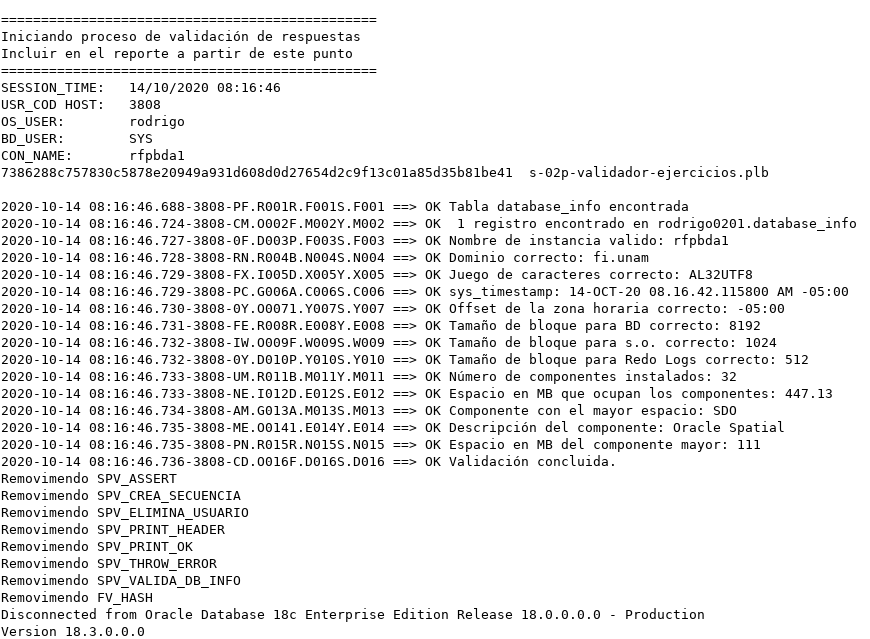
\includegraphics[width=\linewidth]{tema02-ej-prac-01-validador}

\section*{C5. Comentarios y conclusiones}

Los datos obtenidos me permitieron reconocer las vistas y tablas que el manejador
utiliza para almacenar información de la base de datos. Dicha información
será de mucha utilidad en prácticas posteriores  a la hora de crear scripts 
dinámicos para generar una base de datos desde cero.
Por otra parte, parte del trabajo de un DBA es conocer la base de datos
que esta administrando por lo cual esta práctica se vuelve importante.\\ 

Por último, aprendí a utilizar la doble comilla en sentencias 
\texttt{execute immediate}, lo cual me será de utilizad en prácticas 
posteriores. En lugar de utilizar el simbolo \texttt{"}, utilicé el simbolo
dos comillas simples. 

\renewcommand\refname{Bibliografía y referencias}
\begin{thebibliography}{99}
    \bibitem{oracle} Oracle. \textit{Choosing a Character Set} 
    Database Globalization Support Guide en 
    \texttt{https://docs.oracle.com/database/121/NLSPG/ch2charset.htm\#NLSPG002}
    \bibitem{burleson} Burleson Consulting. \textit{Oracle tips } en 
    \texttt{http://www.dba-oracle.com/oracle\_news/}
\end{thebibliography}

\end{document}
